\documentclass{article}

% \usepackage{showframe}
\usepackage[utf8]{inputenc}
\usepackage[T1]{fontenc}
\usepackage{mathptmx}
\usepackage{graphicx}
\usepackage{amsmath}
\usepackage[table]{xcolor}
\usepackage{multirow}
\usepackage{geometry}
 \geometry{
 a5paper,
 left=25mm,
 right=15mm,
 top=25mm,
 bottom=15mm, 
 }
 
% \title{}
% \author{}
% \date{}
% 
% \pdfinfo{%
%   /Title    ()
%   /Author   ()
%   /Creator  ()
%   /Producer ()
%   /Subject  ()
%   /Keywords ()
% }

\renewcommand{\baselinestretch}{1.0}
\makeatletter
\renewcommand\normalsize{\@setfontsize\normalsize{11}{15}}
\renewcommand\large{\@setfontsize\large{13}{15}}
\makeatother

\begin{document}

\begin{center}
 \large{\textbf{BAB II}}\\
 \large{\textbf{TEORI PENUNJANG}}\\
\end{center}
\vspace{2pt}

\noindent \textbf{1.1 Robot Vision}

Robot vision adalah robot yang mampu menggunakan kamera sebagai sumber informasi untuk diolah sesuai kebutuhan (Ude,2010).
Tujuan utama setiap perancangan robot tentu adalah untuk mengganti pekerjaan manusia.
Kemampuan robot untuk melakukan pekerjaan yang berulang dan berbahaya telah menjadi kebutuhan di setiap lingkungan industri (Chao,2014) . 
Untuk memenuhi kebutuhan tersebut telah dikembangkan beragam teknologi sensor dan actuator.
Khusus untuk sensor, telah dikembangkan teknologi yang mirip dengan cara kerja pada indra manusia.
Salah satu yang banyak dipakai adalah penggunaan kamera sebagai pengganti mata untuk robot (Browning,2013).
\\
\noindent \textbf{1.1.1 Robot}

Robot adalah sistem otomasi tingkat lanjut yang menggunakan komputer sebagai bagian dari sistem kendalinya yang terintegrasi (Koren,2010).
Secara umum, robot memiliki setidaknya 3 bagian penting yaitu sensor, sistem kendali, dan akuator.
Sistem kendali dapat berupa sistem analog (berbasis Op-Amp) maupun sistem digital (berbasis chip tertanam atau komputer).
Sensor robot sendiri juga dapat berupa informasi analog maupun digital.
Sedangkan akuator robot sendiri beragam tergantung kebutuhan mulai dari derajat kebebasan satu hingga belasan.
Berikut adalah diagram umum dari robot:
\begin{center}
 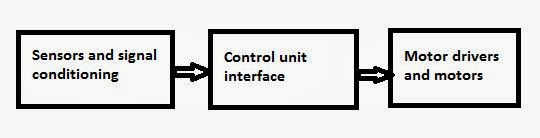
\includegraphics[width=300pt]{general_diagram}
\end{center}

\noindent \textbf{1.1.2 Fungsi Robot}

Fungsi Robot secara umum adalah untuk menggantikan tugas-tugas manusia.
Tugas-tugas manusia tersebut digantikan karena sebab sebagai berikut (Kapila,1990):

\begin{enumerate}

 \item Pekerjaan tersebut berbahaya jika dilakukan oleh manusia. 
 Sebagai contoh pekerjaan di medan berradiasi tinggi, luar angkasa, dan semacamnya.
 \begin{center}
 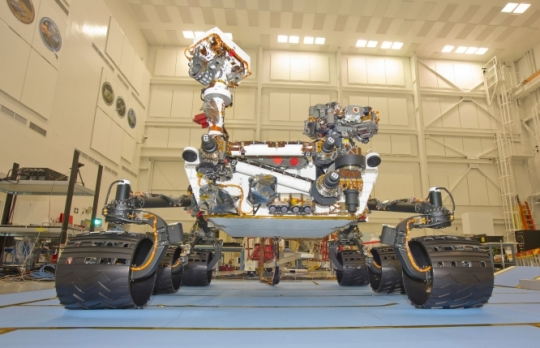
\includegraphics[width=200pt]{mars}
\end{center}

\item Pekerjaan tersebut adalah pekerjaan yang berulang terus-menerus.
Pekerjaan yang bersifat berulang-ulang apabila dikerjakan oleh manusia akan menjadi turun kualitas hasilnya seiring waktu.
Pekerjaan tersebut juga akan menyebabkan manusia kelelahan baik secara fisik dan psikologi.
Sebagai contoh pekerjaan industri seperti perakitan, pengelasan, dan semacamnya.
 \begin{center}
 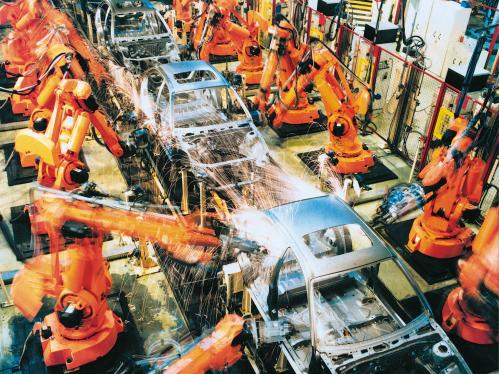
\includegraphics[width=200pt]{industrial_robots}
\end{center}

\item Pekerjaan tersebut memang tidak harus dikerjakan oleh manusia.
Seperti telah diketahui bahwa robot dan mesin pada umumnya hanya membutuhkan maintenance.
Robot tidak memerlukan makan rutin, gaji tetap, tunjangan akhir bulan, asuransi dan semacamnya.
Selain itu robot akan mematuhi perintah dan bekerja dengan kualitas yang cenderung konstan.
Maka dengan menggunakan robot pada pekerjaan tersebut maka tingkat hasil pekerjaan akan meningkat dan biaya semakin mengecil.
Sebagai contoh pekerjaan ini adalah pelayan kantor, pembersih lantai, dan semacamnya.
\begin{center}
 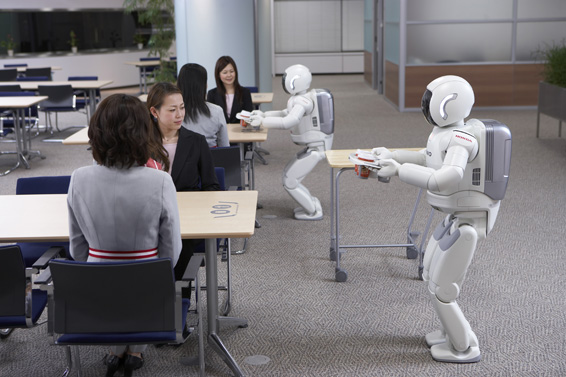
\includegraphics[width=200pt]{help_human}
\end{center}

\end{enumerate}

\noindent \textbf{1.1.3 Sensor Robot}
\\
\noindent \textbf{1.1.4 Aktuator Robot}
\\
\noindent \textbf{1.1.5 Controller Robot}
\\
\\
\vspace{2pt}

\noindent \textbf{1.2 Kamera Digital}
\\
\noindent \textbf{1.2.1 Sensor Kamera Digital}
\\
\noindent \textbf{1.2.2 Data Kamera Digital}
\\
\noindent \textbf{1.2.3 Kelebihan Kamera Digital}
\\
\vspace{2pt}

\noindent \textbf{1.3 Mode Warna}
\\
\noindent \textbf{1.3.1 Citra Digital}
\\
\noindent \textbf{1.3.2 Mode Warna RGB}
\\
\noindent \textbf{1.3.3 Mode Warna HSV}
\\
\vspace{2pt}

\noindent \textbf{1.4 Color Tracking}
\\
\noindent \textbf{1.4.1 Segmentasi}
\\
\noindent \textbf{1.4.2 Citra Biner}
\\
\noindent \textbf{1.4.3 Model Matematis}
\\
\vspace{2pt}

\noindent \textbf{1.5 RapberryPi}
\\
\noindent \textbf{1.5.1 Arsitektur}
\\
\noindent \textbf{1.5.2 Raspbian}
\\
\noindent \textbf{1.5.2 Debian Paket Manager}
\\
\vspace{2pt}

\noindent \textbf{1.6 OpenCV}
\\
\noindent \textbf{1.6.1 Pengolahan Citra}
\\
\noindent \textbf{1.6.2 QtSerialPort}
\\
\vspace{2pt}

\noindent \textbf{1.7 Aktuator}
\\
\noindent \textbf{1.7.1 STM32}
\\
\noindent \textbf{1.7.2 ChibiOS/RT}
\\
\noindent \textbf{1.7.3 Geared Motor DC}
\\
\noindent \textbf{1.7.4 Driver H-Bridge }
\\
\vspace{2pt}

\newpage
.\\
\vspace{200pt}

\hspace{75pt} Halaman ini memang kosong

\end{document}
